\documentclass[UTF8]{gapd}
\usepackage{geometry}%调整页边距
\usepackage{amsmath}%数学
\usepackage{xfrac}%分式
\usepackage{graphicx}%图片
\usepackage{fancyhdr}%页眉
\usepackage{bm}%黑体
\usepackage{hyperref}%生成pdf目录
\usepackage{mathtools}
\usepackage{tensor}%张量
\usepackage{caption}
\usepackage{booktabs}
\usepackage{float}
%基础模板,引用自GitHub: https://github.com/RocketshipGames/gapd.cls

% ■ ■ ■ ■ ■ ■ ■ ■ ■ ■ ■ ■ ■ ■ ■ ■ ■ ■ ■ ■ ■ ■ ■ 
% ■ ■ ■ ■ ■ ■ ■ ■ ■ ■ ■ ■ ■ ■ ■ ■ ■ ■ ■ ■ ■ ■ ■
% ■ ■               注意事项                 ■ ■
% ■ ■      不要瞎几把模板里面cls文件!!!!!   ■ ■
% ■ ■      写着不需要改动的地方别瞎几把动!!!   ■ ■
% ■ ■      有不懂的地方就直接联系编辑!!!!!   ■ ■
% ■ ■      不要自作主张!!!!!!             ■ ■
% ■ ■      否则后续排版会非常累的!!!!!!!   ■ ■
% ■ ■ ■ ■ ■ ■ ■ ■ ■ ■ ■ ■ ■ ■ ■ ■ ■ ■ ■ ■ ■ ■ ■
% ■ ■ ■ ■ ■ ■ ■ ■ ■ ■ ■ ■ ■ ■ ■ ■ ■ ■ ■ ■ ■ ■ ■

%标题部分=================================================================
%上标(不需要改动!!!!)
\Type{Article}

%标题
\Title{
  隐形
}

\CAuthor{杜溪翔}{华中科技大学物理实验创新基地}%显示于题目下的作者名,
\Author{Du Xixiang}{}
%出现于页脚初的英文名,按“姓 名”的顺序写拼音

%摘要
\Abstract{本篇文章所研究的物理现象来源于2021年IYPT(国际青年物理学家竞赛),该题目也作为2021年CUPT(全国大学生物理学术竞赛)中南赛区题目.笔者作为参赛成员参与了本题的部分工作,将结果展示在此.}
\Keywords{透镜组,组合光学,光阑,几何光学}
%编号与页码(以下两行不需要改动)
\Issue{2}{1}{2022}
\Pages{1}{3}%37
%不要改这里,好吗?

%正文部分=================================================================
\begin{document}
%\begin{CJK}{UTF8}{gbsn}
\maketitle

%一些常用的Latex语句:
%插入斜体:\textit{}
%引用文字:\begin{quote} \end{quote}
%插入脚标: \footnote{}

\section{简介}
\label{sec:Introduction}
Lenticular lenses can be used to distort light and make objects disappear. Investigate how changing the properties of the lens and the geometry of the object affect the extent to which the object can be detected.

透镜组可以用来扭曲光线并使物体消失,研究改变透镜的属性和物体的几何形状会如何影响物体被检测到的范围.

%插入图表一定要注意规范!!!!!!!!!!!!!!!!!!!!!!!!!!!!!!!!!!!!!!
%表格一律用三线表,如果有出现数据,请注明数据的单位,另外表格的标题等也要注明清楚。

%插入任何非原创图片都应当注意注明出处
%插入一般的曲线图,一定要注明坐标轴的含义!!!!!及其单位!!!!!!  格式一律为:      物理量 (单位)
%                                                                              ^
%                                                                              |
%                                                                              |
%                                                                              |
%                                                                例子:         ——————————————————————————>
%                                                                                     摆线长度  (mm)
%当图中存在多个曲线,或者数据与拟合图同时存在时,要写清楚图例!!!!!!!!!
%要善于运用跨列图片,把多个相似的子图拼组合成一张比较大的跨列图片

\section{探究流程}
\begin{figure}[htbp]
  \centering
  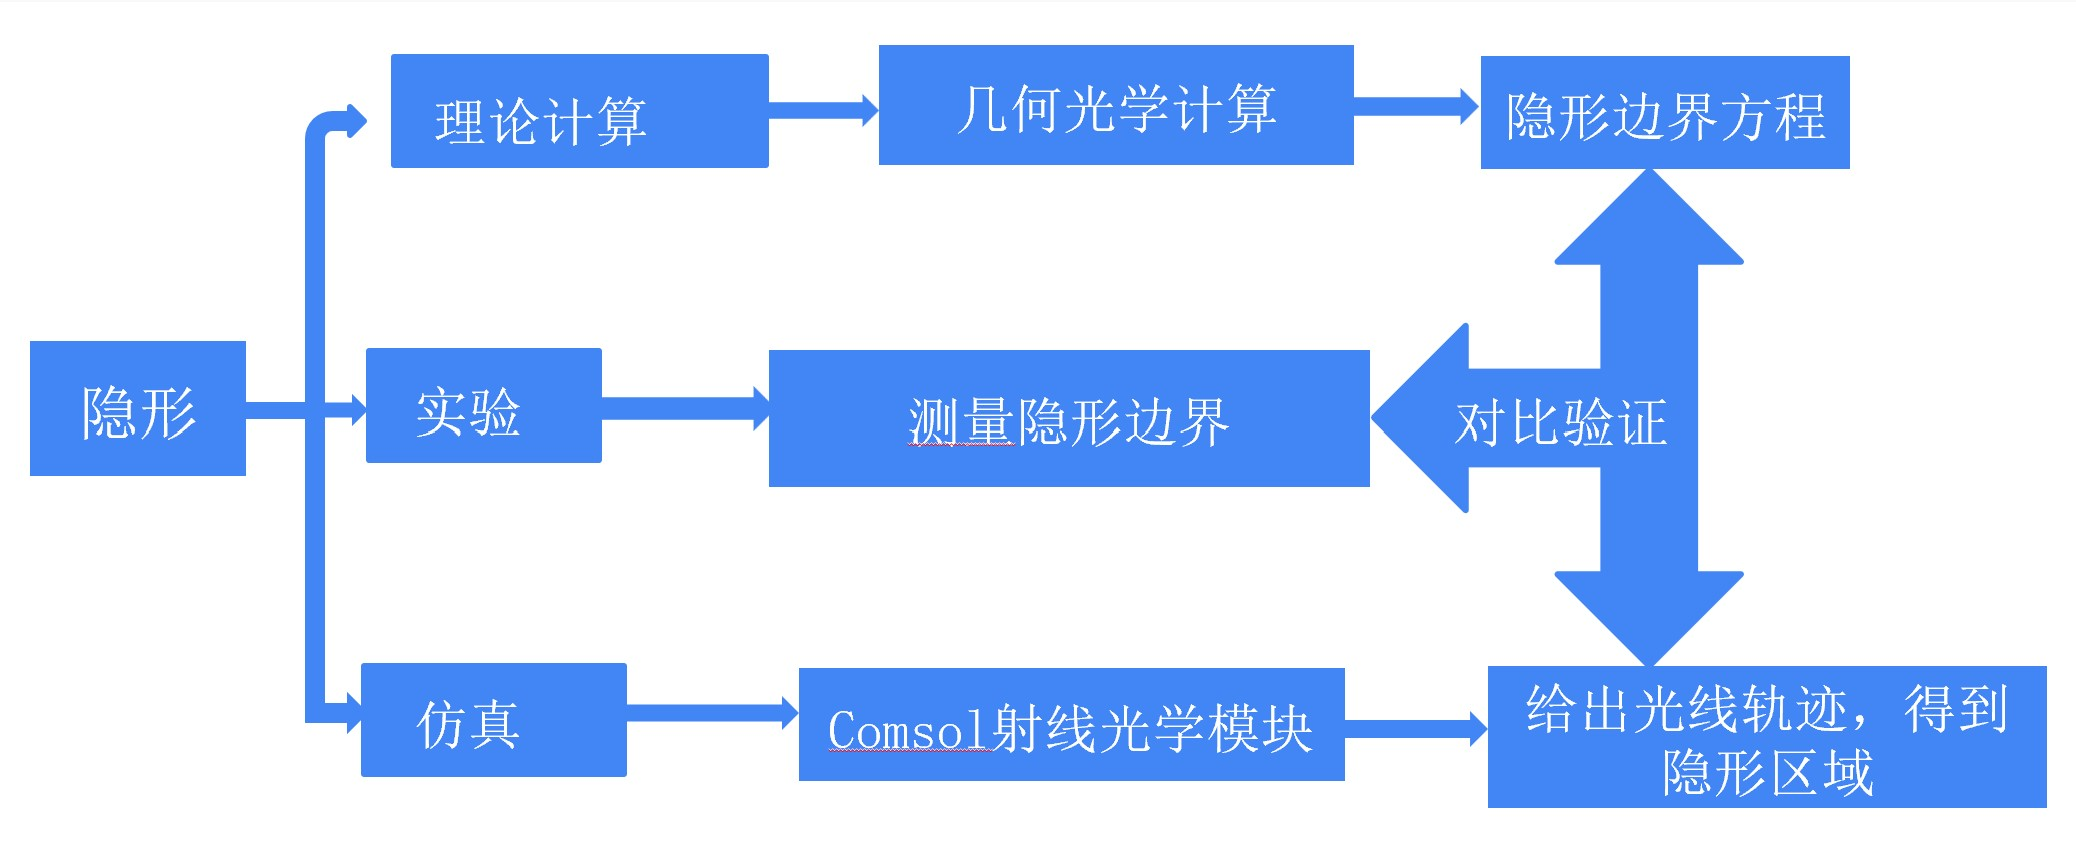
\includegraphics[width=0.4\textwidth]{images/1.jpg}
  \caption{探究流程图}
  \label{fig:1}
\end{figure}
\section{理论}
基本假设:
\begin{enumerate}
  \item 由于实验中透镜直径与延光轴的线度相比很小,在理论计算中采用的傍轴近似可以得到很好的满足.
  \item 用手机的长焦摄像头接受像,故像屏可以认为是一个点,对其作光路可逆分析可以作为点光源.
\end{enumerate}

隐形包含两方面的要求:
\begin{enumerate}
  \item 要求透镜组的成像效果等效与光在空气中不受干扰地传播.
  \item 要求光线在透镜组中传播会绕过障碍物所处的位置,即障碍物反射的光无法被观察者观察到.
\end{enumerate}
\begin{figure}
  \centering
  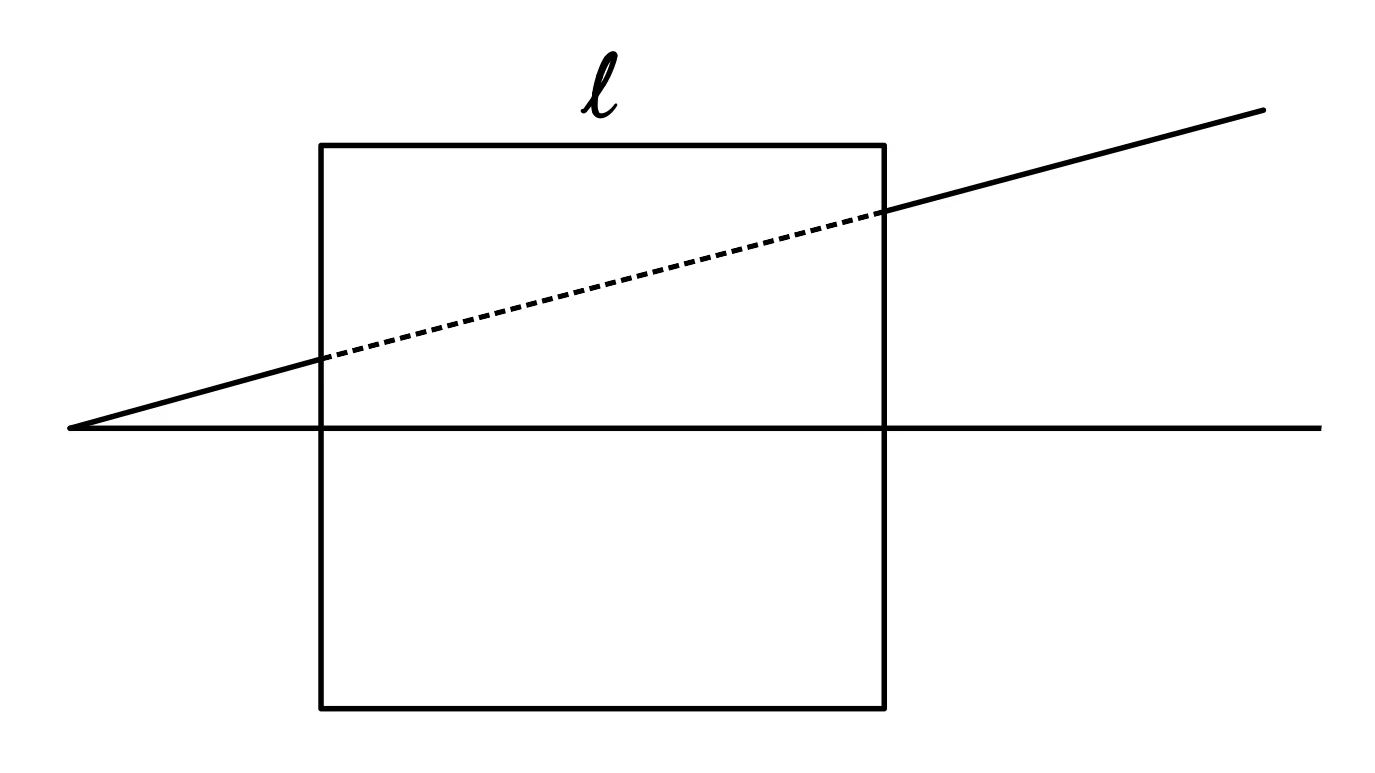
\includegraphics[width=0.4\textwidth]{images/2.jpg}
  \caption{透镜组成像效果与等同于光线在空气中传播}
  \label{fig:2}
\end{figure}
\begin{figure}
  \centering
  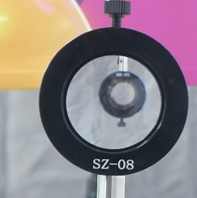
\includegraphics[width=0.4\textwidth]{images/3.jpg}
  \caption{隐形效果图}
\end{figure}
经过数学计算,在1,2,3个透镜的情况下无法实现隐形,对于5,6,7个透镜的情况,则此时也能实现隐形效果.对于更多的透镜,均可以分解为4,5,6,7个透镜的透镜组的组合,即对于4个以上的透镜,均可以实现隐形的效果.

在均匀介质中的传播矩阵和薄透镜的变换矩阵分别为:
\begin{equation}
  M_{Air}=
  \begin{bmatrix}
      1 & L\\
      0 & 1
  \end{bmatrix} ,\quad M_{Len}=\begin{bmatrix}
    1 & 0\\
    -\frac{1}{f} & 1
\end{bmatrix}  
\end{equation}
对于四个透镜的情况:
\begin{figure}
  \centering
  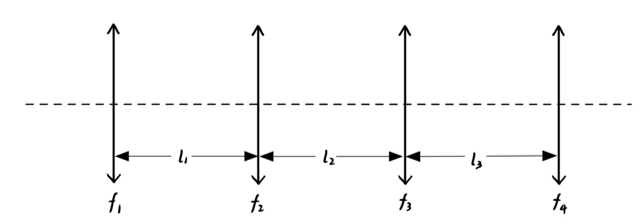
\includegraphics[width=0.4\textwidth]{images/4.png}
  \caption{四透镜情况}
\end{figure}
\begin{multline}
  M=
  \begin{bmatrix}
      1 & 0\\
      -\frac{1}{f_1} & 1
  \end{bmatrix}\begin{bmatrix}
      1&l_1\\
      0&1
  \end{bmatrix}\begin{bmatrix}
      1 & 0\\
      -\frac{1}{f_2} & 1
  \end{bmatrix}\begin{bmatrix}
      1&l_2\\
      0&1
  \end{bmatrix}\\
  \begin{bmatrix}
      1 & 0\\
      -\frac{1}{f_3} & 1
  \end{bmatrix}\begin{bmatrix}
      1&l_3\\
      0&1
  \end{bmatrix}\begin{bmatrix}
      1 & 0\\
      -\frac{1}{f_4} & 1
  \end{bmatrix}\\
  =\begin{bmatrix}
      1&l_1+l_2+l_3\\
      0&1
  \end{bmatrix}
\end{multline}
考虑对称光学系统:
\begin{equation}
  f_4=f_1,\quad f_3=f_2,\quad l_3=l_1
\end{equation}
解得:
\begin{align}
  l_1&=f_1+f_2\\
  l_2&=\frac{2(f_1f_2+f_2^2)}{f_1-f_2}
\end{align}
以上条件满足后,光线经过透镜组折射的效果等同于光线在空气中传播.

下面我们考虑第二点要求,为此,先计算透镜组的光阑,透镜的半径均为$r$,对应孔径光阑的半径为$r'$:
\begin{figure}[htbp]
  \centering
  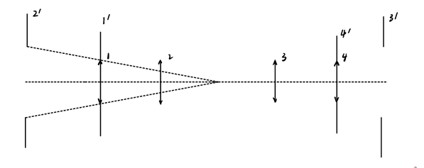
\includegraphics[width=0.4\textwidth]{images/5.jpg}
  \caption{透镜光阑}
  \label{fig:5}
\end{figure}
各个透镜的光阑相对透镜4的位置:
\begin{multline}
    l'_1=-\frac{2f_1(f_1+f_2)}{f_1-f_2} ,\quad l'_2=-\frac{f_1(f_1+f_2)^2}{f_2(f_1-f_2)} ,\\
    l'_3=\frac{f_1(f_1+f_2)}{f_2} 
\end{multline}
\begin{equation}
  r'_1=r,\quad r'_2=r'_3=\frac{f_1}{f_2}d 
\end{equation}
各个光阑对镜头的孔径角分别为:
\begin{align}
  \tan\theta _1&=\frac{r}{u+|l'_1|} ,\quad \\
  \tan\theta _2&=\frac{f_1r}{f_2(u+|l'_2|)} ,\quad \\
  \tan\theta _4&=\frac{r}{u} 
\end{align}
存在关系:
\begin{equation}
  \theta_1<\theta_4
\end{equation}
因此通过透镜4观察,总能看到透镜1的边缘.

$\theta_2$与$\theta_4$的大小关系与镜头到透镜4的距离$u$有关,当:
\begin{equation}
  u>u_1=\frac{f_1(f_1+f_2)^2}{(f_1-f_2)^2} 
\end{equation}
有:
\begin{equation}
  \theta_2>\theta_4
\end{equation}
此时从透镜4中观察,无法观察到透镜2的边缘,此时透镜组的光阑只有1'和2'

当:
\begin{equation}
  u<u_1=\frac{f_1(f_1+f_2)^2}{(f_1-f_2)^2} 
\end{equation}
有:
\begin{equation}
  \theta_2<\theta_4
\end{equation}
此时从透镜4中观察,能够观察到透镜2的边缘.

根据镜头对透镜4所成像在透镜34之间或是透镜23之间,分为两种情况,$u$的临界值为$u_2$,由下式确定:
\begin{equation}
  \frac{1}{u_2}+\frac{1}{l_1}=\frac{1}{f_1},\quad l_1=f_1+f_2   
\end{equation}
解得:
\begin{equation}
  u_2=\frac{f_1(f_1+f_2)}{f_2} 
\end{equation}
下面分情况求解光线方程:

1.$u>u_2$
\begin{figure}
  \centering
  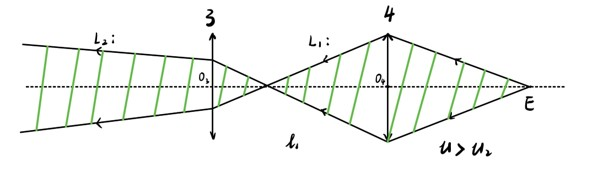
\includegraphics[width=0.4\textwidth]{images/6.jpg}
  \caption{$u>u_2$情况边界示意图}
  \label{fig:6}
\end{figure}
先求直线$L_1$的方程,考虑过透镜边缘的光线,在透镜4右侧,光线的参量为$(y,\theta)=(r,\theta_0)$,经过透镜4后:
\begin{equation}
  \begin{bmatrix}
      y\\
      \theta 
  \end{bmatrix}=\begin{bmatrix}
      1 & 0\\
      -\frac{1}{f_1}  & 1
  \end{bmatrix}
  \begin{bmatrix}
      r\\
      \theta_0 
  \end{bmatrix}=
  \begin{bmatrix}
      r\\
      \theta_0-\frac{r}{f_1} 
  \end{bmatrix}
  ,\quad \theta_0=\frac{r}{u} 
\end{equation}
以透镜4的光心$O_4$为原点向左建立坐标系,则直线$L_1$的方程为:
\begin{equation}
  y=r\big[1-(\frac{1}{f_1}-\frac{1}{u}  )x\big]
\end{equation}
下面求直线$L_2$的方程,在透镜3右侧光线的参量为:
\begin{equation}
  \begin{bmatrix}
      y\\
      \theta
  \end{bmatrix}=
  \begin{bmatrix}
      r[-1+(\frac{1}{f_1}-\frac{1}{u}  )l_1]\\
      r(\frac{1}{f_1}-\frac{1}{u}  )
  \end{bmatrix}
\end{equation}
经过透镜3的变换:
\begin{multline}
  \begin{bmatrix}
    y\\
    \theta
\end{bmatrix}=
\begin{bmatrix}
    1 & 0\\
    -\frac{1}{f_2}  & 1
\end{bmatrix}
\begin{bmatrix}
r [-1+(\frac{1}{f_1}-\frac{1}{u}  )l_1]\\
    r(\frac{1}{f_1}-\frac{1}{u}  )
\end{bmatrix}   \\
=
\begin{bmatrix}
    r(\frac{f_2}{f_1}-\frac{f_1+f_2}{u}  )\\
    \frac{rf_1}{uf_2} 
\end{bmatrix}
\end{multline}
以透镜3的光心$O_3$为原点向左建立坐标系,光线$L_2$的方程为:
\begin{equation}
  y=r(\frac{f_2}{f_1}-\frac{f_1+f_2}{u}+\frac{f_1}{uf_2}x   )
\end{equation}

2.$u<u_2$
\begin{figure}
  \centering
  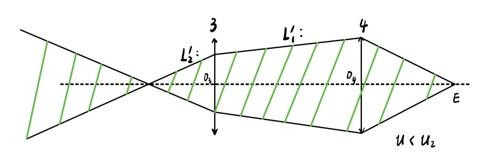
\includegraphics[width=0.4\textwidth]{images/7.jpg}
  \caption{$u<u_2$情况边界示意图}
  \label{fig:7}
\end{figure}
下面求直线$L_1'$和直线$L_2'$方程,由于变换矩阵与前一种情况完全相同,故所求出的直线方程也与上一种情况相同,分别以透镜光心$O_4$,$O_3$为原点向左建立坐标系,直线$L_1'$方程为:
\begin{equation}
  y=r\big[1-(\frac{1}{f_1} -\frac{1}{u} )x\big]
\end{equation}
直线$L_2'$方程为:
\begin{equation}
  y=r(\frac{f_1+f_2}{u}-\frac{f_2}{f_1}-\frac{f_1}{uf_2}x   )
\end{equation}
下面讨论透镜12之间的隐形区域,此时按照透镜24的光阑的孔径角$\theta_2$,$\theta_4$的大小分类讨论,临界时的$u$由$u_1$给出:
\begin{equation}
  u_1=\frac{f_1(f_1+f_2)^2}{(f_1-f_2)^2} >u_2
\end{equation}
$u>u_1$时,临界光线仍为经过透镜4边缘的光线:
\begin{figure}
  \centering
  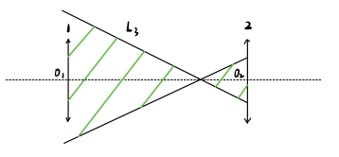
\includegraphics[width=0.4\textwidth]{images/8.jpg}
  \caption{$u>u_1$情况边界示意图}
\end{figure}
该光线在透镜12之间区域的方程为$L_3$,下面求直线$L_3$的方程.设光线在透镜2左侧的参量为$(y_1,\theta_1 )$:
\begin{equation}
  \begin{bmatrix}
      1 & 0\\
      -\frac{1}{f_1} & 1
  \end{bmatrix}
  \begin{bmatrix}
      1&l_1\\
      0&1
  \end{bmatrix}
  \begin{bmatrix}
      y_1\\
      \theta_1
  \end{bmatrix}=
  \begin{bmatrix}
      1 & 2l_1+l_2\\
     0 & 1
  \end{bmatrix}
  \begin{bmatrix}
      r\\
      \frac{r}{u} 
  \end{bmatrix}
\end{equation}
解得:
\begin{equation}
  \begin{bmatrix}
      y_1\\
      \theta_1
  \end{bmatrix}=\begin{bmatrix}
      -r[\frac{f_2}{f_1}+\frac{(f_1+f_2)^2}{f_1-f_2}\frac{1}{u}   ]\\
      r(\frac{1}{f_1}+ \frac{3f_1+f_2}{f_1-f_2}\frac{1}{u}  )
  \end{bmatrix}
\end{equation}
则$L_3$方程为:
\begin{equation}
  y=r[-\frac{f_2}{f_1}-\frac{(f_1+f_2)^2}{f_1-f_2}\frac{1}{u}  + (\frac{1}{f_1}+ \frac{3f_1+f_2}{f_1-f_2}\frac{1}{u}  )x]
\end{equation}
当$u<u_1$,临界光线为经过透镜2边缘的光线:
\begin{figure}
  \centering
  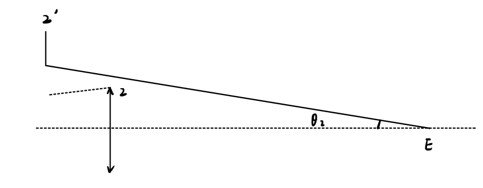
\includegraphics[width=0.4\textwidth]{images/9.jpg}
  \caption{物象共轭原理}
  \label{fig:9}
\end{figure}
\begin{figure}
  \centering
  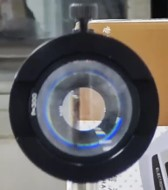
\includegraphics[width=0.4\textwidth]{images/10.jpg}
  \caption{透镜元件自身带有光阑}
  \label{fig:10}
\end{figure}
根据物像共轭的原理经过透镜2边缘的光线在像方的延长线经过光阑2',倾角:
\begin{equation}
  \theta_2=\frac{r'_2}{|l'_2|+u} =\frac{rf_1/f_2}{u+f_1(f_1+f_2)^2/(f_1-f_2)^2} 
\end{equation}
设此时透镜12间隐形边界方程为$L_3'$,为了求$L_3'$,只需将$L_3$方程中:
\begin{equation}
  r\rightarrow \theta_2 u
\end{equation}
得到$L_3'$方程:
\begin{equation}
  y=\theta_2u[-\frac{f_2}{f_1}-\frac{(f_1+f_2)^2}{f_1-f_2}\frac{1}{u}  + (\frac{1}{f_1}+ \frac{3f_1+f_2}{f_1-f_2}\frac{1}{u}  )x]
\end{equation}
\begin{equation}
  \theta_2=\frac{r'_2}{|l'_2|+u} =\frac{rf_1/f_2}{u+f_1(f_1+f_2)^2/(f_1-f_2)^2} 
\end{equation}
经过计算,不论$u$取何值,在透镜12间的隐形区域都是V形区域.
\paragraph{理论部分小节}
\begin{enumerate}
  \item $0<u<f_1$时,在视场中能看到三个透镜的边缘,每个透镜的光阑都对光线有约束,隐形区域过小,不讨论这种情况.
  \begin{figure}[htbp]
    \centering
    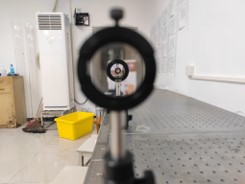
\includegraphics[width=0.4\textwidth]{images/11.jpg}
    \caption{该情况隐形区域过小}
    \label{fig:11}
  \end{figure}
  \item $f_1<u<u_2$时,有效光阑为1',2',4',透镜34间的隐形区域为直线型$(L_1')$,透镜23间的隐形区域为V型$(L_2')$,透镜12间的隐形区域为V型$(L_3)$.
  \begin{figure}[htbp]
    \centering
    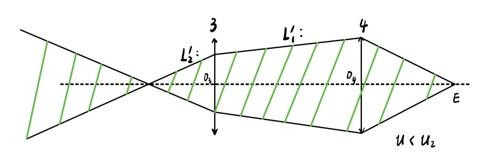
\includegraphics[width=0.4\textwidth]{images/12.jpg}
    \caption{$f_1<u<u_2$情况边界示意图}
    \label{fig:12}
  \end{figure}
  \begin{figure}[htbp]
    \centering
    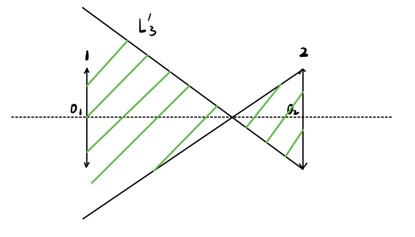
\includegraphics[width=0.4\textwidth]{images/13.jpg}
    \caption{$f_1<u<u_2$情况边界示意图}
    \label{fig:13}
  \end{figure} 
  \item $u_2<u<u_1$时,有效光阑为1',2',4',透镜34间的隐形区域为V型($L_1$) ,透镜23间的隐形区域为直线型$(L_2)$,透镜12间的隐形区域为V型$(L_3)$.
  \begin{figure}[htbp]
    \centering
    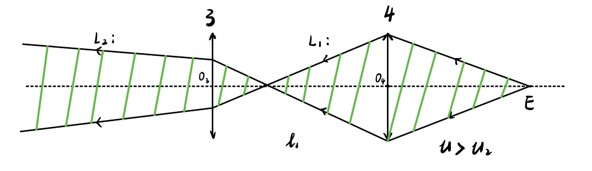
\includegraphics[width=0.4\textwidth]{images/14.jpg}
    \caption{$u_2<u<u_1$情况边界示意图}
    \label{fig:14}
  \end{figure}
  \begin{figure}[htbp]
    \centering
    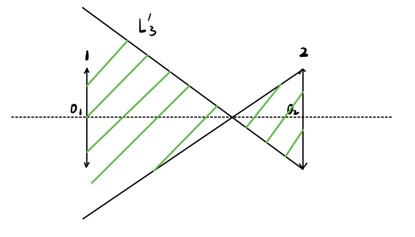
\includegraphics[width=0.4\textwidth]{images/15.jpg}
    \caption{$u_2<u<u_1$情况边界示意图}
    \label{fig:15}
  \end{figure}
  \item $u_1<u$时.有效光阑为1', 4',透镜34间的隐形区域为V型$(L_1)$,透镜23间的隐形区域为直线型$(L_2)$,透镜12间的隐形区域为V型$(L'_3)$.
  \begin{figure}[htbp]
    \centering
    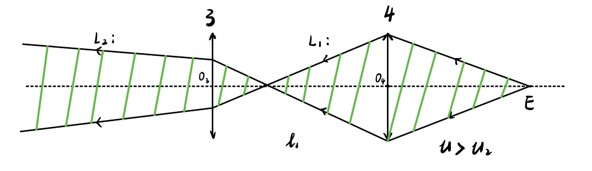
\includegraphics[width=0.4\textwidth]{images/16.jpg}
    \caption{$u_1<u$情况边界示意图}
    \label{fig:16}
  \end{figure}
  \begin{figure}[htbp]
    \centering
    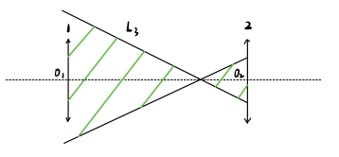
\includegraphics[width=0.4\textwidth]{images/17.jpg}
    \caption{$u_1<u$情况边界示意图}
  \end{figure}
\end{enumerate}
\section{实验}
\label{sec:Experiment}
\begin{figure}[htbp]
  \centering
  
\includegraphics[width=0.4\textwidth]{images/18.jpg}
  \caption{实验流程}
  \label{fig:18}
\end{figure}
\begin{figure}[htbp]
  \centering
  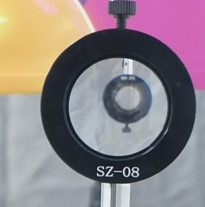
\includegraphics[width=0.3\textwidth]{images/19.jpg}
  \caption{隐形效果}
  \label{fig:19}
\end{figure}
\begin{figure}[htbp]
  \centering
  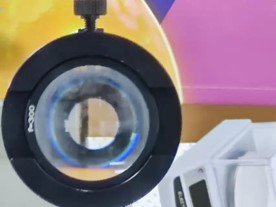
\includegraphics[width=0.4\textwidth]{images/20.jpg}
  \caption{隐形效果}
  \label{fig:20}
\end{figure}
\begin{figure}[H]
  \centering
  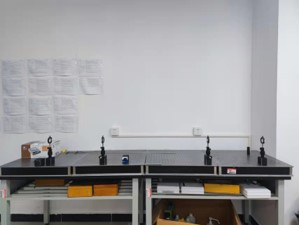
\includegraphics[width=0.4\textwidth]{images/21.jpg}
  \caption{实验平台}
  \label{fig:21}
\end{figure}
\begin{figure}[H]
  \centering
  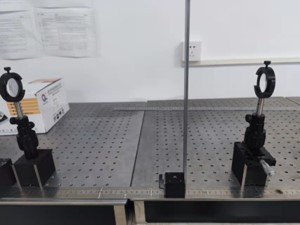
\includegraphics[width=0.4\textwidth]{images/22.jpg}
  \caption{实验平台}
  \label{fig:22}
\end{figure}
\begin{figure}[htbp]
  \centering
  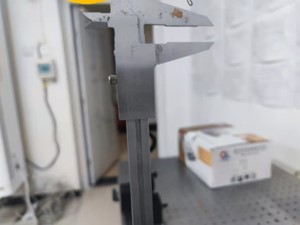
\includegraphics[width=0.4\textwidth]{images/23.jpg}
  \caption{测量间距器材}
  \label{fig:23}
\end{figure}
\begin{figure}[htbp]
  \centering
  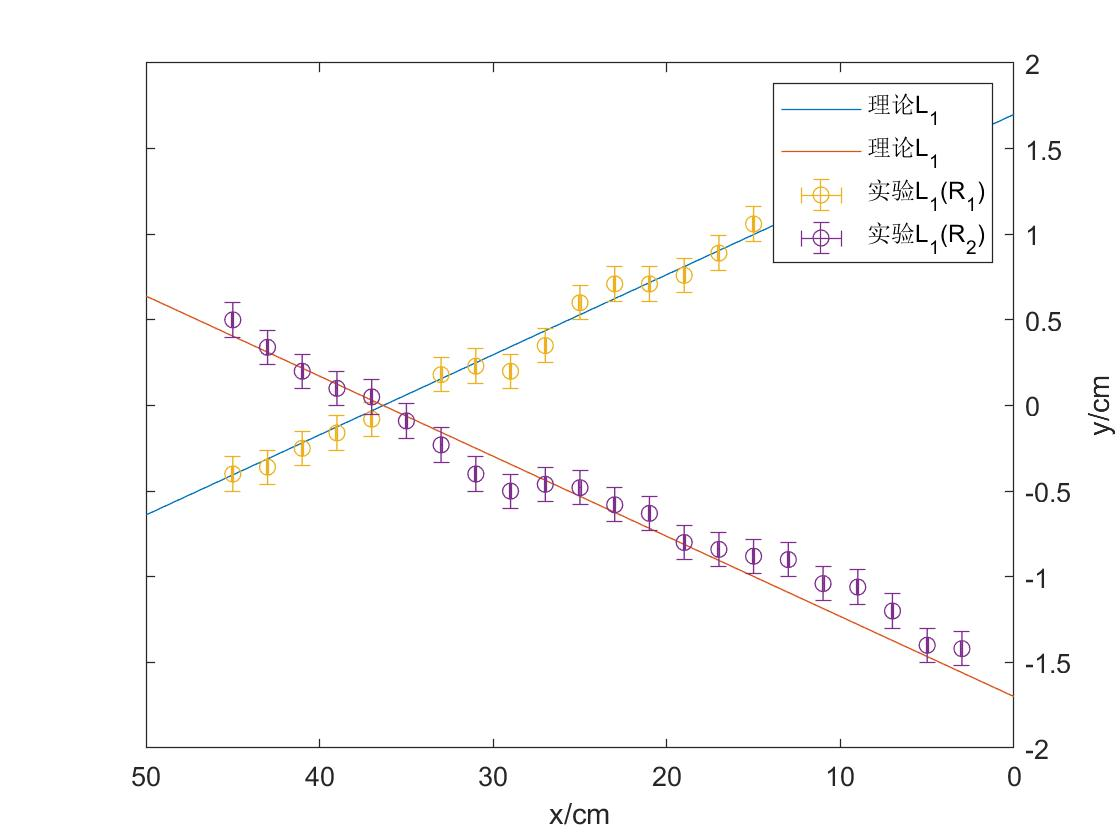
\includegraphics[width=0.4\textwidth]{images/24.jpg}
  \caption{透镜34之间区域 $R_1^2=0.9866,R_2^2=0.9600$}
\end{figure}
\begin{figure}[htbp]
  \centering
  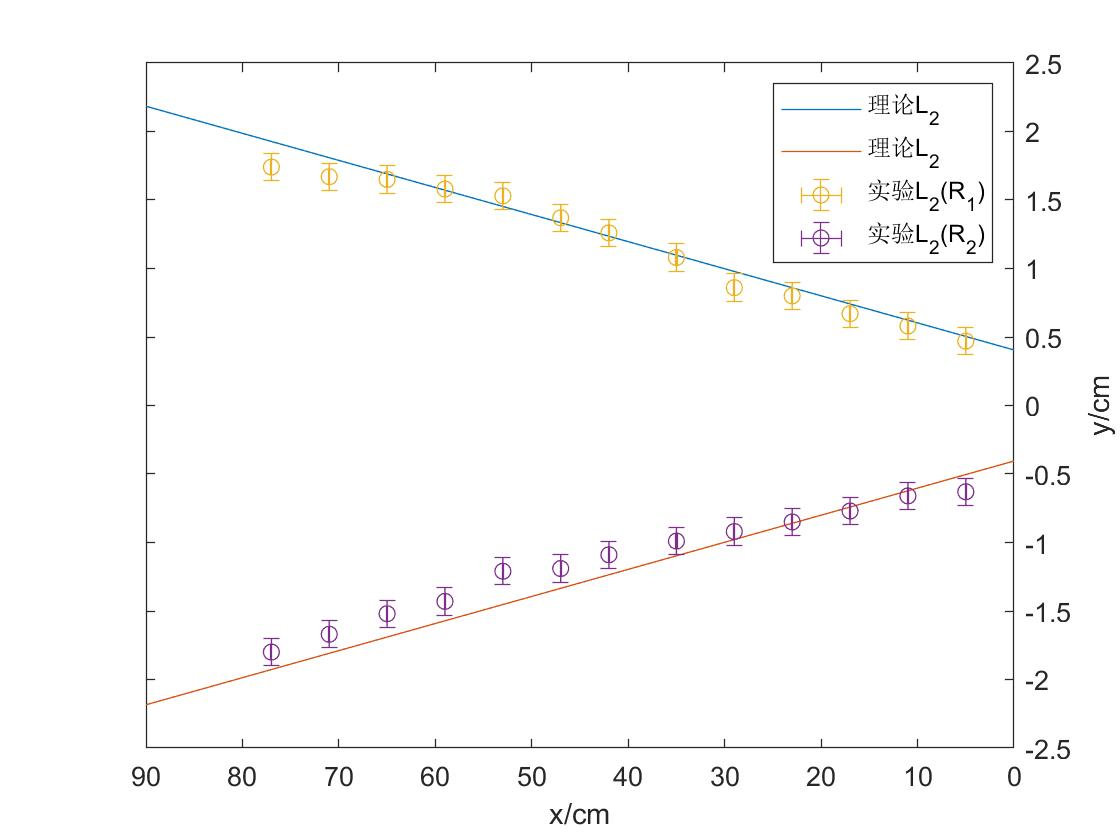
\includegraphics[width=0.4\textwidth]{images/25.jpg}
  \caption{透镜23之间区域$R_1^2=0.9638,R_2^2=0.8742$}
\end{figure}
\begin{figure}[htbp]
  \centering
  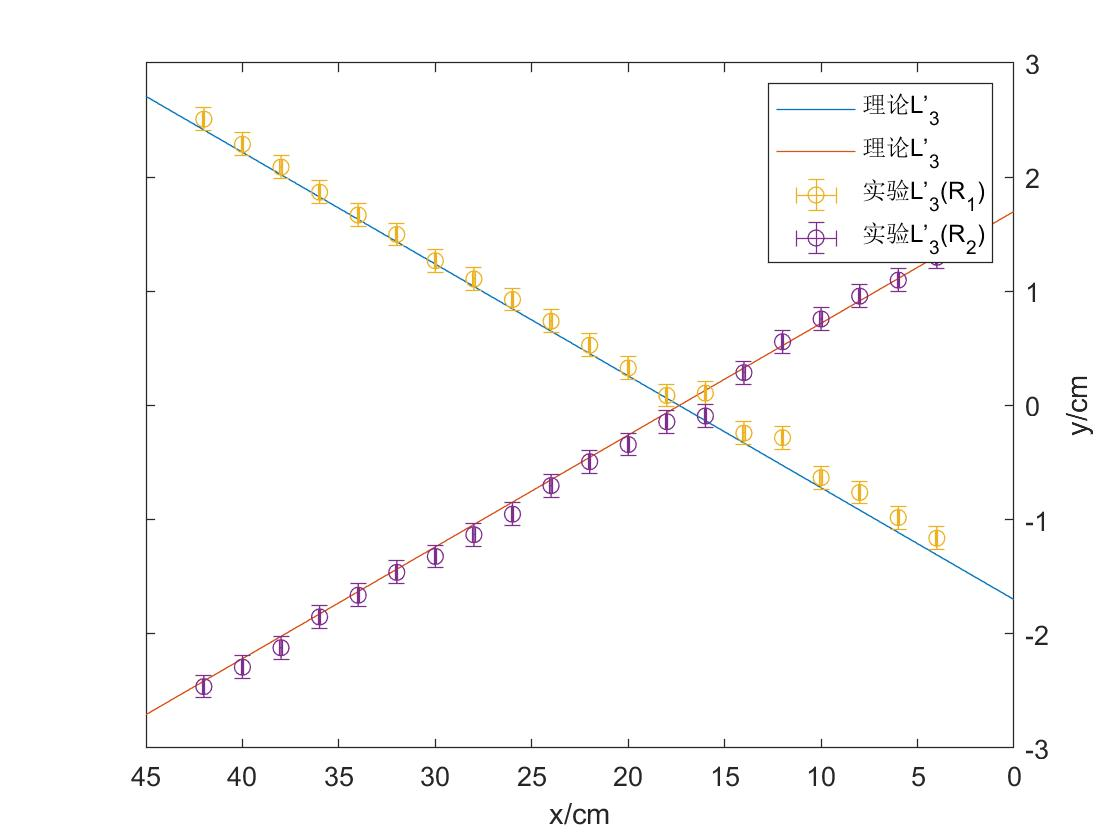
\includegraphics[width=0.4\textwidth]{images/26.jpg}
  \caption{透镜12之间区域$R_1^2=0.9896,R_2^2=0.9955$}
\end{figure}
\section{误差分析}
误差来源:
\begin{enumerate}
  \item 傍轴近似.
  \item 色散效应,自然光包含不同波长的光,不同波长的光线并不重合.
\end{enumerate}
\paragraph{傍轴近似产生误差的数量级估计}
傍轴近似产生的误差来源于以下近似:
\begin{equation}
  \sin\theta \approx \theta
\end{equation}
若精确到三阶项:
\begin{equation}
  \sin\theta \approx \theta -\frac{1}{6}\theta ^3 
\end{equation}
相对偏差:
\begin{equation}
  U=\frac{1}{6}\theta ^2 
\end{equation}
$\theta$取透镜孔径对焦点的张角:
\begin{equation}
  \theta=\frac{d}{f} \sim \frac{3.41\mathrm{cm} }{15\mathrm{cm} }= 0.23
\end{equation}
\begin{equation}
  U=\frac{1}{6}\theta ^2=1\%
\end{equation}
\paragraph{色散效应产生误差的数量级估计}
磨镜者公式:
\begin{equation}
  f=\frac{1}{(n-1)(\frac{1}{r_1}+\frac{1}{r_2}  )} 
\end{equation}
则有:
\begin{equation}
  \frac{|\Delta f|}{f} =\frac{|\Delta n|}{n-1} 
\end{equation}
可见光波长400~780nm,根据成都光明公司的光学玻璃数据表,对于冕牌玻璃K9L:
\begin{align*}
  n(\lambda_h=404.66\mathrm{nm} &=1.530251),\\
  n(\lambda_r=706.52\mathrm{nm} &=1.512901),\\
  \Delta n&=0.01735
\end{align*}
\begin{equation}
  \frac{\Delta f}{f}=\frac{0.01735}{1.5168-1}=4\%  
\end{equation}
\section{仿真部分}
\begin{figure}[htbp]
  \centering
  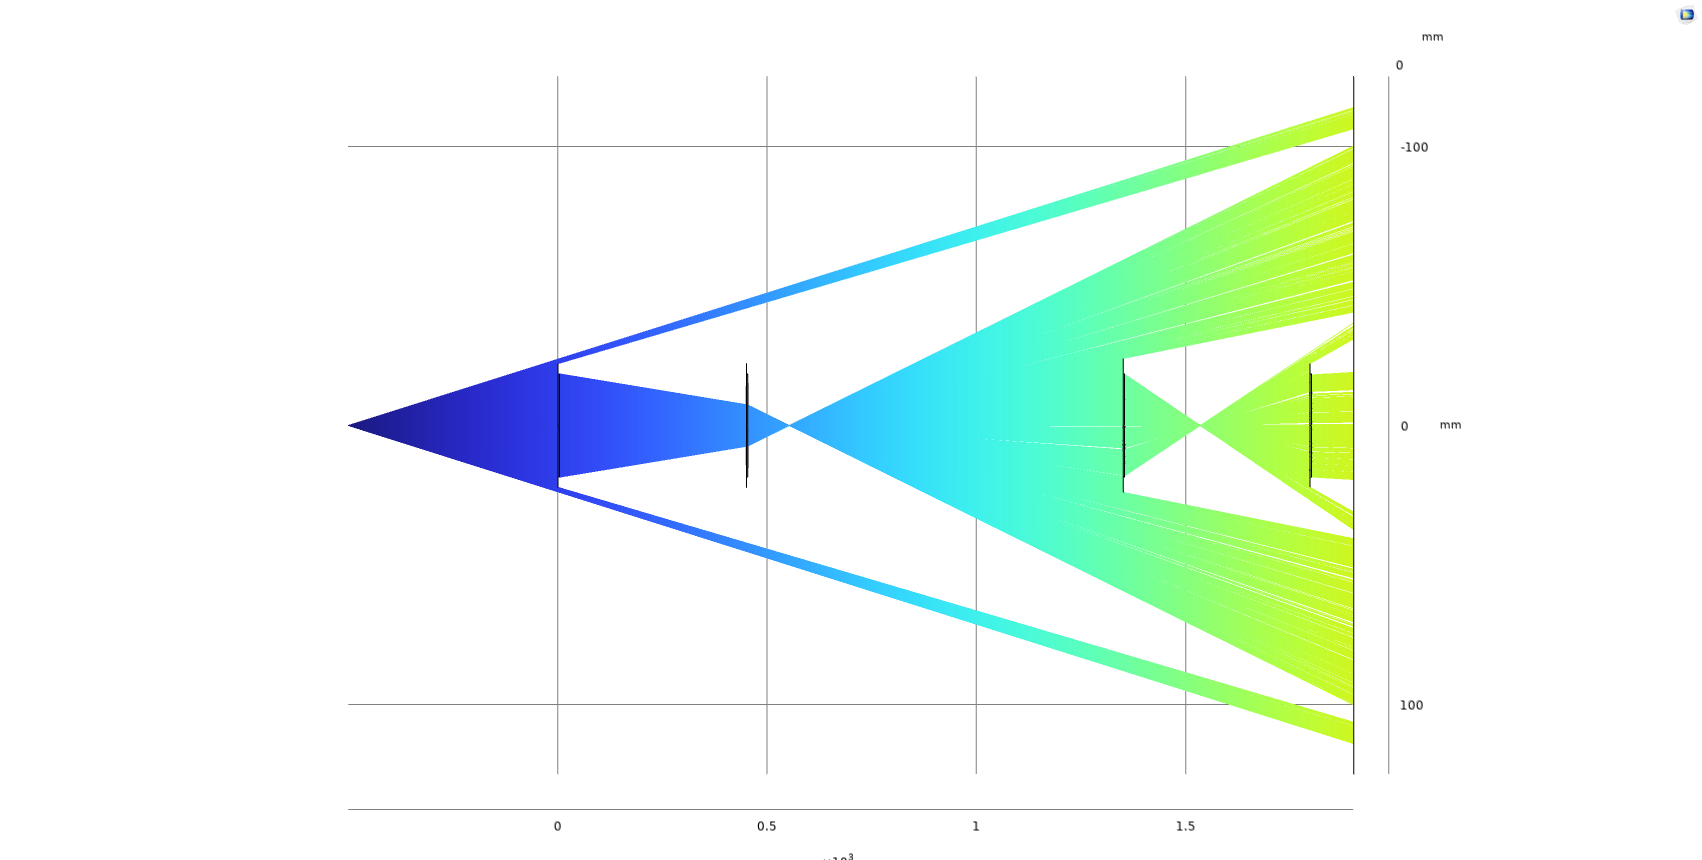
\includegraphics[width=0.4\textwidth]{images/27.png}
  \caption{$u=50\mathrm{cm} $}
\end{figure}
\begin{figure}[htbp]
  \centering
  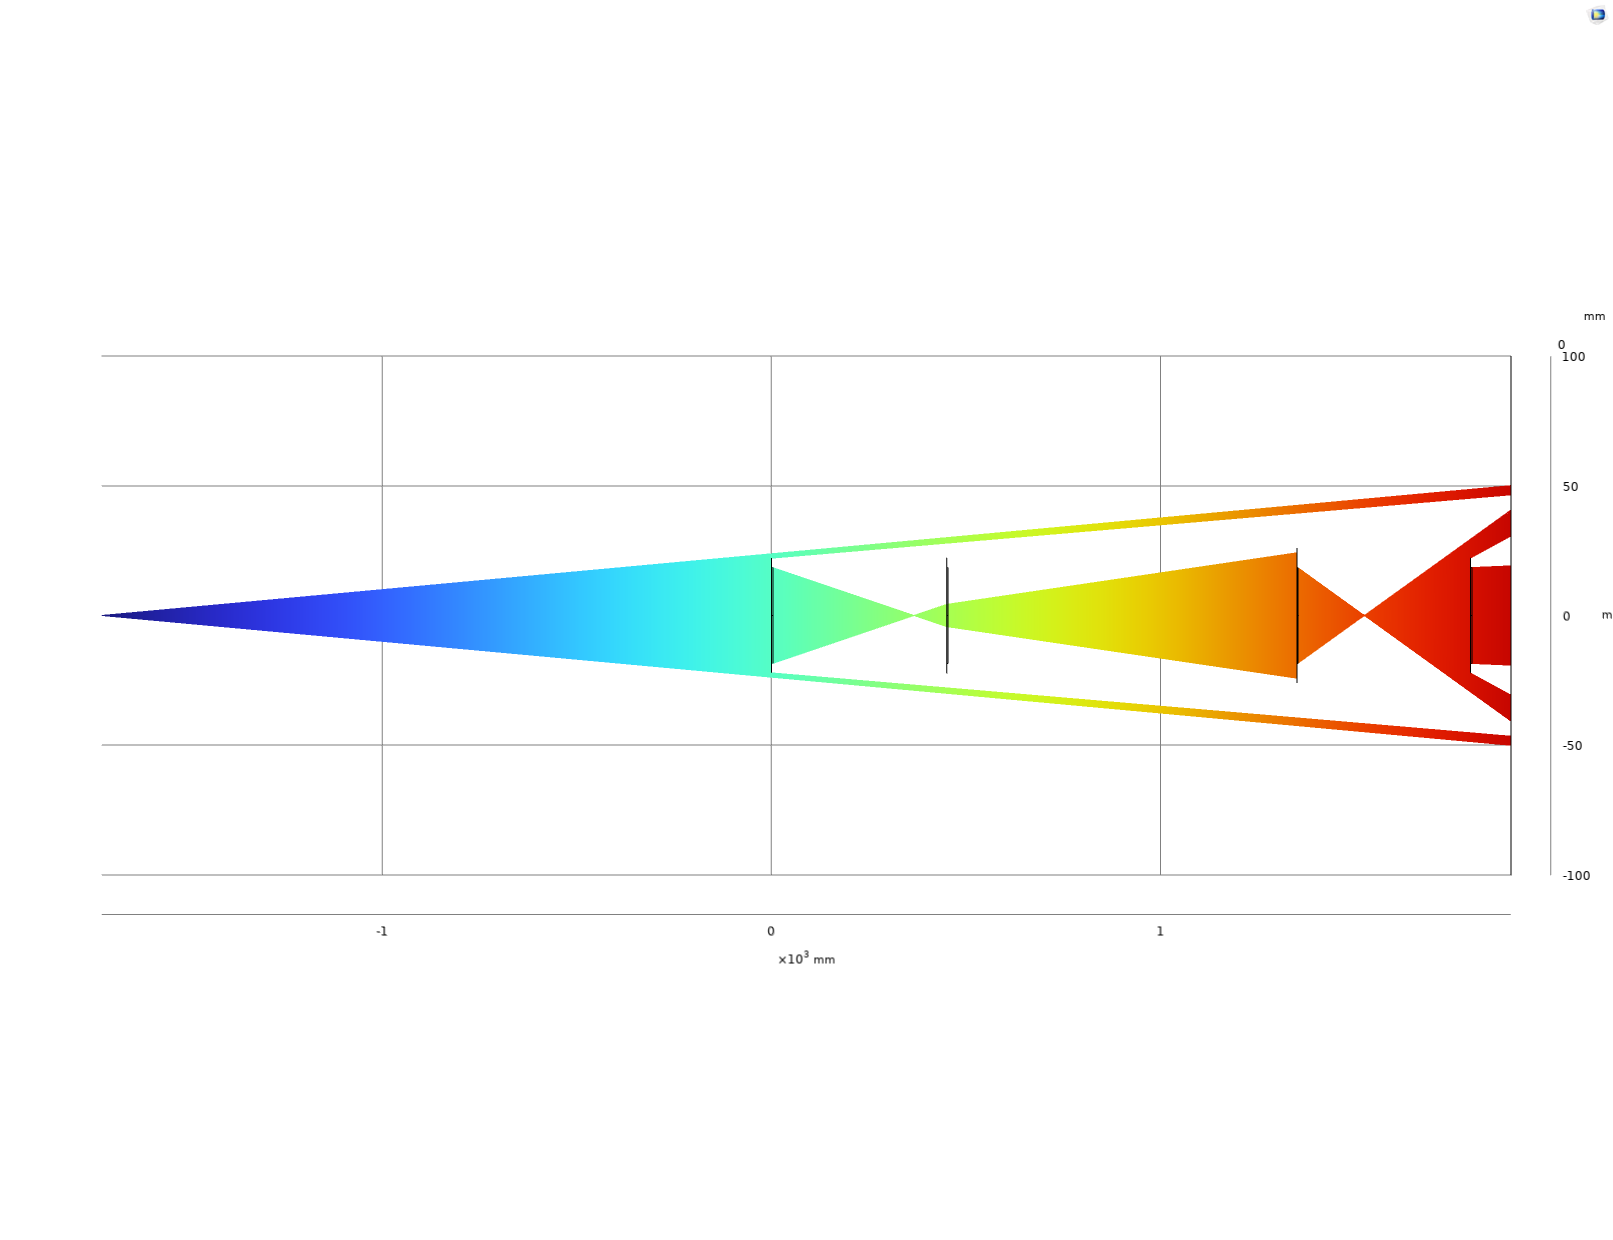
\includegraphics[width=0.4\textwidth]{images/28.png}
  \caption{$u=172\mathrm{cm} $}
\end{figure}
\begin{figure}[htbp]
  \centering
  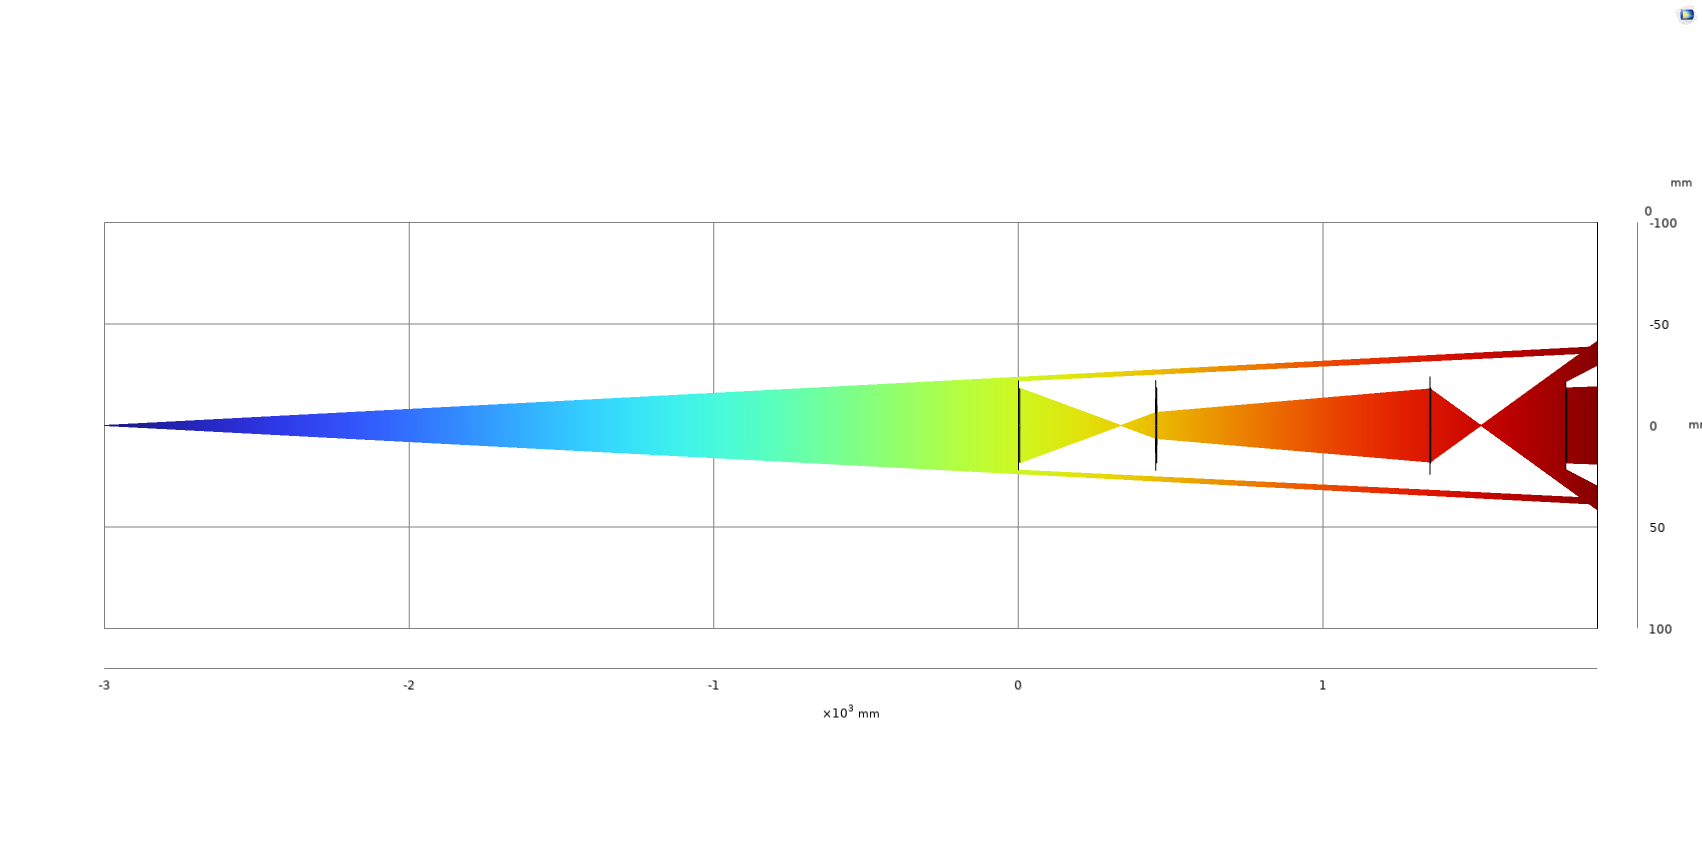
\includegraphics[width=0.4\textwidth]{images/29.png}
  \caption{$u=300\mathrm{cm} $}
\end{figure}
\section{结论}
\begin{enumerate}
  \item 理论上证明了四个及四个以上的透镜可以形成隐形现象,并具体讨论四个透镜的情况.
  \item 在傍轴近似的条件下通过矩阵光学的理论方法得到隐形的边界方程.隐形的范围与透镜的几何参数和观察距离𝑢有关.通过分类讨论得到了不同情况下的边界方程.
  \item 实验和仿真与理论符合得很好,验证了理论的正确性.
\end{enumerate}
\section{展望}
\begin{enumerate}
  \item 对傍轴近似进行更精细定量的考虑,考虑更高阶的像差,如球差,慧差,像散,场曲,畸变.
  \item 考虑光的波动性的影响,如艾里斑.
\end{enumerate}
%致谢,参考文献与背景信息部分=========================================================
\section*{致谢}
小组成员:杜溪翔,苏佳诺,符镫之,任权东.感谢物理实验创新基地(IBPE)的各成员的协作.感谢师兄师姐提供的建议与帮助.感谢北京大学物理学院杨天睿同学,部分图片出于他手.


%背景信息
\Note{BlueNoteBackground}{
  {\textbf{Your Name}} is the chief editor of IBPE Rev. Lett.\\
  {\textbf{Address:}} School of Physics, Huazhong University of Science and Technology\\
  {\textbf{Email:}} IBPE@hust.edu.cn
}


\section*{参考文献}
\begin{thebibliography}{2}

\bibitem{c1}王晨阳,陈柏良,何新,杨俊波.关于四透镜近轴光学隐身区域的探讨[J].中阿科技论坛(中英文),2020(12):102-105.

\bibitem{c2}张化雨,王泽冠,张家浩,彭惠宁,孙腊珍,张增明,王中平.利用简单透镜组实现近轴光学隐身[J].物理实验,2016,36(10):37-40.

\end{thebibliography}

%\end{CJK}
\end{document}
